%%%%%%%%%%%%%%%%%%%%%%%%%%%%%%%%%%%%%%%%%%%%%%%%%%%%%%%%%%%%%%%%%%
\section{Accuracy and cost on benchmark problems}\label{sec:accuracy_cost}
%%%%%%%%%%%%%%%%%%%%%%%%%%%%%%%%%%%%%%%%%%%%%%%%%%%%%%%%%%%%%%%%%%
% Streams feeding this section: R4 (Hron-Turek FSI3) and R6 (blobInTreacle).
% The 2D block with a flexible tail (Jaiman and Joshi 2022) has no case in
% solids4foam (A1 Section 1.14); it is added only if Philip approves it at G1.

A coupling is more efficient than another only if it reaches the same accuracy at lower cost.
This section compares the complete quasi-monolithic and partitioned IQN-ILS solver formulations under matched meshes and time steps (their discretisations differ in the ways listed in Section~\ref{sec:consistency_partitioned}), and reports the error against the reference together with the cost, as a work--precision relation.

%%--------------------------------------------------------------------------------------------------------------------%%
\subsection{Hron--Turek FSI3}\label{sec:fsi3_m}
% TIME-SCHEME NOTE (Philip, 22 Oct 2026), for anyone adding results here:
% all transient results in this paper must use BDF2 (backward) for the fluid
% ddt(U) and the solid. The solids4foam tutorial default for this case is
% backward for the fluid ddt(U). Confirm and record the ddt schemes of every
% run (runs.csv); rerun any result computed with Euler, and say so here.
\todo{Time scheme: confirm that every result in this subsection uses BDF2 (backward) for the fluid and the solid (tutorial default at \texttt{a421f063d}: backward for both regions); results computed with Euler must be rerun.}
%%--------------------------------------------------------------------------------------------------------------------%%
% Set-up: companion paper sectionBenchmarkSuite.tex "Hron--Turek family";
% solids4foam 257b2e564 tutorials/fluidSolidInteraction/TurekHron2006/
% verification/README.md section "Quasi-monolithic coupling" (lines 551-592):
% conformal meshes with a quarter of the tutorial's solid cells (5 x 30 on the
% plate at 1x); dt 0.001 / 0.0005 / 0.00025 s at 1x / 2x / 4x (driver level
% table, A1 Section 1.7); diffusionHyperElastic pseudo-solid stiffened near
% the plate and cylinder. Monolithic solid:
% nonLinearGeometryTotalLagrangianVelocity, direct map.
% Driver: verification/Allverify --coupling monolithic --levels 1,2,4.

The FSI3 problem of~\citet{Turek2006}, an elastic flag behind a rigid cylinder oscillating at a low solid-to-fluid density ratio (Figure~\ref{fig:fsi3_geom_m}), is the most widely used test of strongly coupled FSI solvers, and its Featflow reference values carry an uncertainty of about $3$--$5\%$ in the displacement and force amplitudes and less than $0.3\%$ in the frequency and mean drag~\citetodo{companion verification paper}.

\begin{figure}[htbp]
	\centering
	\includegraphics[scale=1]{figures/HronTurek3-geometry}
	\caption{Hron--Turek FSI3: geometry and monitoring point A.}
	\label{fig:fsi3_geom_m}
\end{figure}
\todo{Replace the mesh in Figure~\ref{fig:fsi3_geom_m} with the conformal-interface mesh used here (carried over from the earlier draft).}

\paragraph{Set-up.}
Both couplings are run on the conformal meshes of the quasi-monolithic set-up at refinement factors 1, 2 and 4, with $\Delta t = 0.001$, $0.0005$ and $0.00025\,\mathrm{s}$ respectively, to $t = \tbd{7}\,\mathrm{s}$; these meshes have a quarter of the solid cells of the companion paper's meshes at each factor.
The flag is computed with the geometrically nonlinear velocity solid (quasi-monolithic) and the displacement solid with IQN-ILS under the strict convergence test (partitioned).
The fluid mesh is moved by a pseudo-solid stiffened near the flag and the cylinder (Section~\ref{sec:fluid_mesh_motion}); with uniform stiffness the fluid mesh inverts during the start-up overshoot at $t = 2.76\,\mathrm{s}$ with either coupling.
% Source of the mesh-inversion statement: TurekHron2006/verification/README.md
% lines 557-562 and commit 415ee9a6d (A4 Section 8, route C). Mesh level not
% stated; ask Philip.
\todo{State the mesh level at which the uniform pseudo-solid inverted (A4 open question 4).}

\paragraph{Measured.}
The mean and amplitude of $u_x$(A), the amplitude and frequency of $u_y$(A), the mean and amplitude of the drag and the amplitude of the lift, over the last \tbd{second}, with the lift smoothed as in the companion paper, and their errors against the Featflow level-4 values.
The cost is timed over two oscillation periods from a periodic restart, with the same number of processes for both couplings at each level.
On the factor-2 mesh the iterative side of the work--precision relation is measured by a tolerance sweep: \texttt{snes\_rtol} of $10^{-4}$, $10^{-6}$ and $10^{-8}$ for the quasi-monolithic coupling and strict coupling tolerances of $10^{-4}$, $10^{-5}$ and $10^{-6}$ for IQN-ILS.

\todo{Figure: FSI3 work--precision, one panel per quantity ($u_x$ mean, $u_y$ amplitude, drag amplitude, lift amplitude; optionally $u_y$ frequency and drag mean). Horizontal axis: core-hours per simulated second (log). Vertical axis: relative error against Featflow level 4 (log). Filled markers: quasi-monolithic; open markers: IQN-ILS; marker shape: refinement factor (1, 2, 4), joined by a line per coupling; small markers on the factor-2 point: tolerance sweep. Shaded horizontal band: reference uncertainty of the companion paper, below which errors cannot be distinguished. Data: R4 \texttt{runs.csv}, \texttt{qois.csv}.}

\todo{Table: FSI3 on the conformal meshes. Rows: factor 1, 2, 4 for each coupling. Columns: fluid and solid cells; $\Delta t$; processes; errors in $u_x$ mean, $u_y$ amplitude, $u_y$ frequency, drag mean, drag amplitude, lift amplitude; Newton or coupling iterations per step; Krylov iterations per Newton iteration; wall time per step; core-hours per simulated second.}

Expected claims: on the same meshes the two couplings give errors that differ by \tbd{value} and approach each other under refinement; at equal error the quasi-monolithic coupling costs \tbd{factor} times \tbd{more/less} than IQN-ILS, and below an error of \tbd{value} the reference uncertainty, not the coupling, limits the comparison.
The observed order of the quasi-monolithic $u_x$ mean between factors 2 and 4 is \tbd{order}, which shows whether the first-order sequence of the companion paper comes from the coupling or from the discretisation and set-up.
% HANDOFF R4 "Order check for V": V cites one sentence on this. Pre-#597
% (stale) errors were 11.5% and 5.9% (README table), about order 1.

%%--------------------------------------------------------------------------------------------------------------------%%
\subsection{Elastic half-cylinder in a viscous channel flow}\label{sec:blob_m}
% TIME-SCHEME NOTE (Philip, 22 Oct 2026), for anyone adding results here:
% all transient results in this paper must use BDF2 (backward) for the fluid
% ddt(U) and the solid. The solids4foam tutorial default for this case is
% Euler for the fluid ddt(U). Confirm and record the ddt schemes of every
% run (runs.csv); rerun any result computed with Euler, and say so here.
% Every run here: fluid ddt(U), ddt(dU), ddt(p) and solid backward (tutorial at a421f063d).
%%--------------------------------------------------------------------------------------------------------------------%%
% Set-up: solids4foam 257b2e564 tutorials/fluidSolidInteraction/
% blobInTreacle/README.md (case overview and parameter table) and
% verification/README.md (time and mesh studies; "Quasi-monolithic
% coupling", lines 195-227); companion paper "Blob in treacle".
% Monolithic solid: linearGeometryVelocity, direct map. No monolithic
% driver: job scripts (A1 Section 1.6). blobInTreacle IS the Liu, Jaiman and
% Gurugubelli (2014) temporal-accuracy case (A1 Section 1.14).

\citet{Liu2014} proposed an elastic half-cylinder attached to the floor of a highly viscous channel flow (Figure~\ref{fig:blob_geom_m}) to measure the temporal order of their quasi-monolithic finite element formulation, on which the present method is based~\citep{JaimanJoshi2022}.
Repeating their temporal study with the present cell-centred finite volume formulation is therefore the most direct comparison with the finite element method; the companion paper uses the case only for a partitioned self-convergence study~\citetodo{companion verification paper}.

\begin{figure}[htbp]
	\centering
	\includegraphics[scale=1]{figures/blobInTreacle-geometry}
	\caption{Elastic half-cylinder in a viscous channel flow: geometry (in m), boundary conditions and top point A; the mesh drawn is finer than the factor-1 mesh.}
	\label{fig:blob_geom_m}
\end{figure}
% Figure checked against the blobInTreacle README and blockMeshDict at a421f063d:
% radius 0.5 m centred at (1.5, -0.5) m in the channel [0, 6.5] x [-0.5, 1] m.

\paragraph{Set-up.}
A linear elastic half-cylinder of radius $0.5\,\mathrm{m}$ ($\lambda_s = 500\,\mathrm{Pa}$, $\mu_s = 50\,\mathrm{Pa}$, $\rho_s = 1\,\mathrm{kg/m^3}$) is attached to the floor of a channel carrying a fluid of the same density and kinematic viscosity $1\,\mathrm{m^2/s}$, so that the Reynolds number is of order one and the added mass is strong.
A parabolic inlet velocity is ramped up over $2\,\mathrm{s}$, after which the flow settles to a steady state.
The solid is the geometrically linear velocity solid, and both regions use BDF2 in time.
% The quasi-monolithic variant uses backward for the fluid and the solid since
% solids4foam 6dc42799b (Euler for the fluid before, e.g. at 257b2e564).

\paragraph{Measured.}
The temporal study follows~\citet{Liu2014} and the partitioned study of the companion paper: on the tutorial mesh (480 fluid and 120 solid cells), $\Delta t = 0.25$ to $0.015625\,\mathrm{s}$, halved each time, to $t = 1\,\mathrm{s}$, with the self-convergence of the top-point displacement $u_x$(A) and of the $\ell_2$ norm of the change in the interface vertex positions.
The quasi-monolithic coupling uses Newton tolerances of $10^{-8}$ and a Krylov tolerance of $10^{-6}$ here, so that its iterative error lies below the smallest change; IQN-ILS uses the strict test with the tutorial tolerance of $10^{-6}$.
The mesh study repeats the steady $u_x$(A) on mesh factors 1, 2 and 4 ($\Delta t = 0.01$, $0.01$ and $0.005\,\mathrm{s}$) to $t = 3\,\mathrm{s}$, by which time $u_x$(A) varies by less than $2\times10^{-4}$ of its value over the last $0.5\,\mathrm{s}$, with the tutorial tolerances.
Both couplings are run serially on the same workstation and build.
% Runs: local Mac Studio, a421f063d-equivalent build, ~/claude-runs/agent-b-blob
% (tutorial driver verification/Allverify); QM rows reproduce the R-fix rows
% (evidence/m-runs-a-rfix) to 7 digits. Partitioned factor 4: WP0
% (evidence/m-runs-wp0, 85b0c1de6, 4 ranks).

\begin{figure}[htbp]
	\centering
	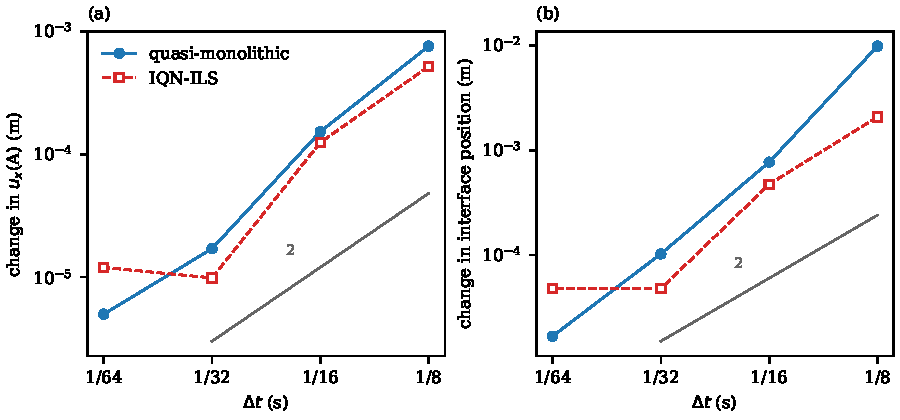
\includegraphics[width=0.9\textwidth]{figures/blobInTreacle-time}
	\caption{Elastic half-cylinder, tutorial mesh, $t = 1\,\mathrm{s}$: successive change in (a) the top-point displacement $u_x$(A) and (b) the interface position ($\ell_2$ norm over the interface vertices) against the finer of the two time steps, quasi-monolithic (Newton tolerance $10^{-8}$) and IQN-ILS (strict test, $10^{-6}$), with a slope of 2.}
	\label{fig:blob_time}
\end{figure}

\paragraph{Temporal convergence.}
The temporal sequence of the quasi-monolithic coupling is broadly compatible with second-order convergence (Figure~\ref{fig:blob_time}): the observed orders of $u_x$(A) are 2.31, 3.17 and 1.77 and those of the interface position 3.68, 2.91 and 2.61, consistent with the second-order self-convergence reported by~\citet{Liu2014} for their finite element formulation.
IQN-ILS converges at a similar rate from the largest steps (orders 2.05 and 3.67 for $u_x$(A), 2.14 and 3.31 for the interface) but stops at an iterative floor of about $10^{-5}\,\mathrm{m}$ in $u_x$(A) and $5\times10^{-5}\,\mathrm{m}$ in the interface position, which its tolerance of $10^{-6}$ sets: below $\Delta t = 0.03125\,\mathrm{s}$ the successive change no longer falls.
Tightening the IQN-ILS tolerance does not remove the floor, as the interface residual then stagnates at about $2.5\times10^{-8}$, the level set by the inner fluid and solid solver tolerances.
The quasi-monolithic coupling needs 2.0--3.0 Newton iterations per step and IQN-ILS 14--24 coupling iterations, and the five quasi-monolithic runs together take $11\,\mathrm{s}$ against $76\,\mathrm{s}$ for IQN-ILS, seven times less, although the quasi-monolithic runs use the tighter tolerances.
At the smallest step the two couplings differ by $0.71\%$ in $u_x$(A), the same as their difference in the steady state on this mesh (Table~\ref{tab:blob_mesh}), which is therefore a spatial and not a temporal difference.

\begin{table}[htbp]
	\centering
	\footnotesize
	\caption{Elastic half-cylinder: steady top-point displacement $u_x$(A) at $t = 3\,\mathrm{s}$ on mesh factors 1, 2 and 4, relative difference between the couplings, observed order, Richardson extrapolation with the observed order, and serial solver time to $t = 3\,\mathrm{s}$.}
	\label{tab:blob_mesh}
	\begin{tabular}{lrrrrr}
		\toprule
		Factor & \multicolumn{2}{c}{$u_x$(A) (m)} & Difference & \multicolumn{2}{c}{Time (s)} \\
		& quasi-monolithic & IQN-ILS & & quasi-monolithic & IQN-ILS \\
		\midrule
		1 & 0.116390 & 0.117260 & $-0.74\%$ & 19 & 148 \\
		2 & 0.119224 & 0.119688 & $-0.39\%$ & 71 & 643 \\
		4 & 0.119991 & 0.120206\textsuperscript{a} & $-0.18\%$ & 947 & --\textsuperscript{a} \\
		\midrule
		Observed order & 1.89 & 2.23 & & & \\
		Extrapolated & 0.120276 & 0.120346 & $-0.06\%$ & & \\
		\bottomrule
	\end{tabular}
	\par\smallskip
	\parbox{0.9\linewidth}{\footnotesize \textsuperscript{a}~From the earlier run of the same set-up on four processes (solids4foam \texttt{85b0c1de6}); on the present build the serial IQN-ILS run reached the limit of 100 coupling iterations in a step at $t = 1.26\,\mathrm{s}$. The factor-1 and factor-2 values of the two builds agree to $2.5\times10^{-4}$ relative.}
\end{table}

\paragraph{Mesh convergence.}
Both couplings converge at close to second order in space (Table~\ref{tab:blob_mesh}), and their steady displacements differ by $0.74$, $0.39$ and $0.18\%$ on the three meshes, halving with each refinement, and by $0.06\%$ after extrapolation, so the two couplings converge to the same solution; this difference is discussed with the other discretisation differences in Section~\ref{sec:consistency_partitioned}.
The quasi-monolithic coupling needs 2.0, 2.0 and 2.6 Newton iterations per step on the three meshes, with 24, 36 and 62 Krylov iterations per Newton iteration, whereas IQN-ILS needs 18 and 26 coupling iterations per step on the two coarser meshes, with steps of up to 86 and 98 iterations; the quasi-monolithic runs are eight to nine times faster.
With equal fluid and solid densities and a viscous flow, the partitioned iterations converge slowly on this case, and the quasi-monolithic coupling gains correspondingly.

\paragraph{Discussion: cost per step and number of iterations.}
A Newton iteration of the quasi-monolithic coupling solves a preconditioned linear system for all fluid and solid unknowns, whereas a coupling iteration of the partitioned schemes performs one segregated fluid solve and one solid solve.
A Newton iteration is therefore the more expensive of the two, and the quasi-monolithic coupling is cheaper per step only when the partitioned scheme needs sufficiently many coupling iterations.
In the cases of this paper the quasi-monolithic coupling needs two to four Newton iterations per step independently of the added-mass ratio (Sections~\ref{sec:ring_m} and~\ref{sec:robustness}), whereas the coupling iterations of the partitioned schemes grow with it.
Measured on the same processes, a Newton iteration costs about as much as 1.2 IQN-ILS coupling iterations on the two-dimensional ring and half-cylinder and about 2.4 on the three-dimensional flag of Section~\ref{sec:lim_foil}, whose fluid block needs more Krylov iterations.
The break-even point is therefore case dependent: the quasi-monolithic coupling is cheaper where the partitioned scheme needs more coupling iterations per step than the number of Newton iterations times this cost ratio, about 2.5--5 in the two-dimensional cases and about 8 on the flag (3.3 Newton iterations per step): by a factor of two on the ring at the strong added-mass level, where IQN-ILS needs 4--6, and by a factor of seven to nine on the half-cylinder, where it needs 14--26.
Where few coupling iterations suffice, as for the flag (5.4 per step) and the steady flexible-bottom cavity (Section~\ref{sec:cavity_m}), the accelerated partitioned schemes are the cheaper choice, by a factor of 1.5 on the flag.
On the Hron--Turek FSI3 benchmark, the only case of the paper with an established external reference and a work--precision comparison, the quasi-monolithic coupling costs \tbd{factor} times \tbd{more/less} than IQN-ILS at equal error (Section~\ref{sec:fsi3_m}).
% Ratios: ring tab:ring_cost (QM step ~0.5 IQN step, 2 Newton vs 4.4-5.6 its);
% blob time study (11 s vs 76 s; 2.0-3.0 Newton vs 14-24 its); foil 8 ranks
% (337 s vs 229 s; 3.3 Newton vs 5.4 its).
